\documentclass{article}
\usepackage{ctex}
\usepackage{color}
\usepackage{listings}
\usepackage{graphicx}
\usepackage{float}
\usepackage{subfig}
\usepackage{overpic}
\lstset{ %
basicstyle=\footnotesize,       % the size of the fonts that are used for the code
numbers=left,                   % where to put the line-numbers
numberstyle=\footnotesize,      % the size of the fonts that are used for the line-numbers
stepnumber=1,                   % the step between two line-numbers. If it is 1 each line will be numbered
numbersep=5pt,                  % how far the line-numbers are from the code
backgroundcolor=\color{white},  % choose the background color. You must add \usepackage{color}
showspaces=false,               % show spaces adding particular underscores
showstringspaces=false,         % underline spaces within strings
showtabs=false,                 % show tabs within strings adding particular underscores
frame=single,           % adds a frame around the code
tabsize=2,          % sets default tabsize to 2 spaces
captionpos=b,           % sets the caption-position to bottom
breaklines=true,        % sets automatic line breaking
breakatwhitespace=false,    % sets if automatic breaks should only happen at whitespace
}

\title{\heiti Specification Document For Painkiller Injection System}
\author{%
  Panxin Tao, Runkang Yang, Zhekai Zhang\\
  SIST, ShanghaiTech University\\
  \texttt{taopx2022@shanghaitech.edu.cn}\\
  \texttt{yangrk2022@shanghaitech.edu.cn}\\
  \texttt{zhangzhk2022@shanghaitech.edu.cn}\\
}
\date{June 2024}
\begin{document}
\maketitle
\newpage
\section{Contents}
\subsubsection{System Architecture}
\subsubsection{Specification}
\newpage
\section{System Architecture}
Below is the architecture of the Painkiller Injection System:
\begin{figure}[htbp]
  \centering
  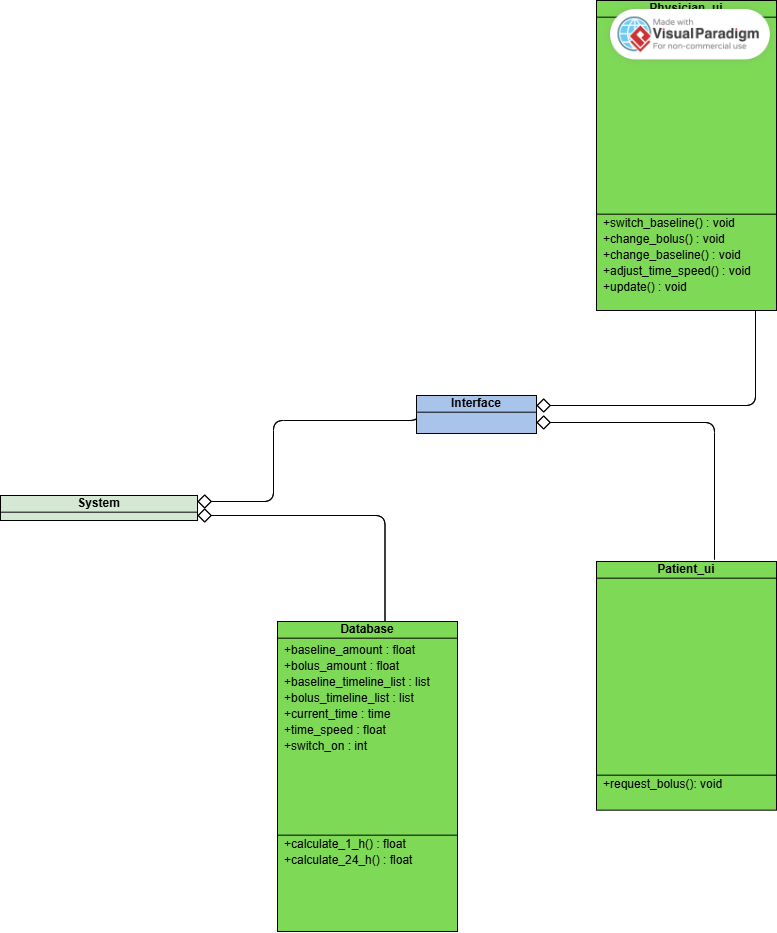
\includegraphics[width=0.8\textwidth]{img/System.png}
  \caption{System Architecture}
\end{figure}
\newpage
\section{Specification}
\subsection*{S1: Physician Operations}
\subsubsection*{S1.1: Adjust Baseline Amount}
\begin{figure}[htbp]
  \centering
  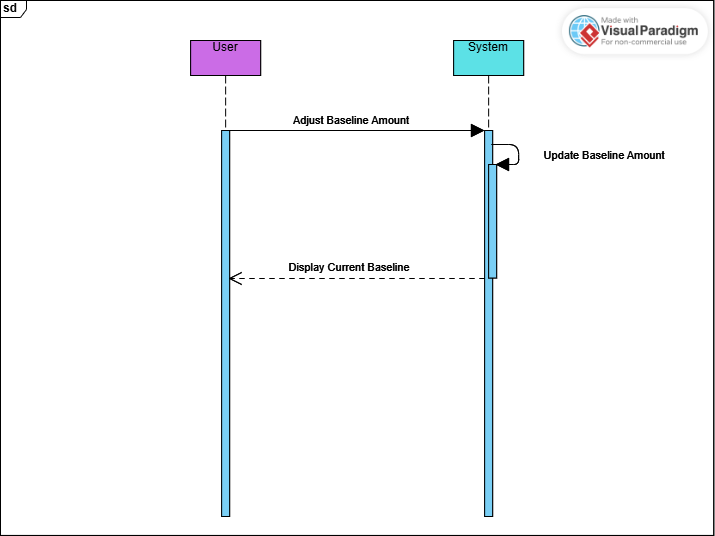
\includegraphics[width=0.8\textwidth]{img/S1_1.png}
  \caption{S1.1}
\end{figure}
Frontend: The user uses the scrollbar to adjust the baseline amount, which ranges from 0.01ml/min to 0.1ml/min.

Backend: \lstinline!database.baseline_amount! changes to the adjusted value.

System Response: The current baseline will be displayed on screen.
\subsubsection*{S1.2: Set Bolus Amount}
\begin{figure}[htbp]
  \centering
  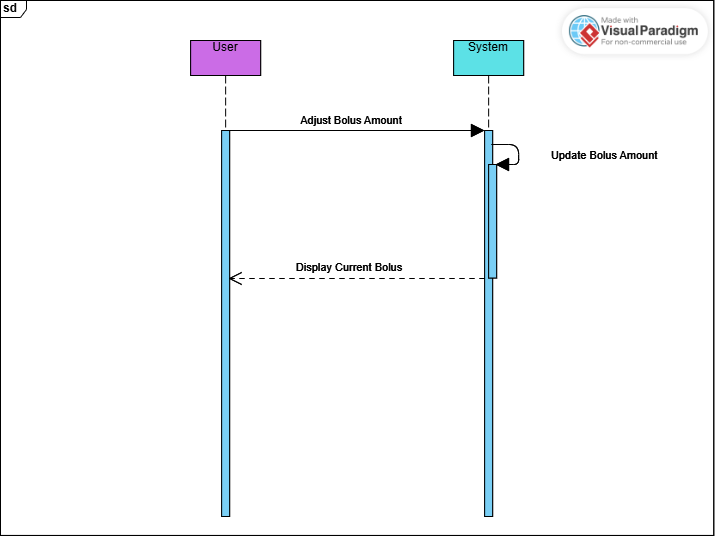
\includegraphics[width=0.8\textwidth]{img/S1_2.png}
  \caption{S1.2}
\end{figure}
Frontend: The user uses the scrollbar to adjust the bolus amount, which ranges from 0.2ml/shot to 0.5ml/shot.

Backend: \lstinline!database.bolus_amount! changes to the adjusted value.

System Response: The current bolus will be displayed on screen.
\subsubsection*{S1.3: Baseline Switch}
\begin{figure}[htbp]
  \centering
  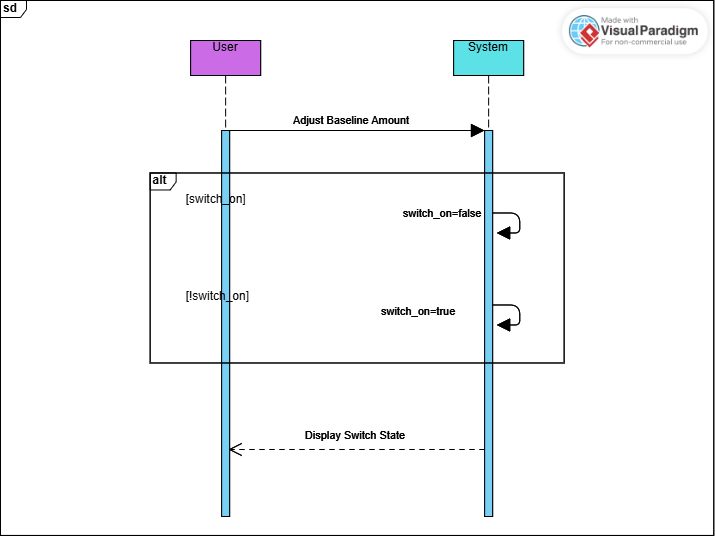
\includegraphics[width=0.8\textwidth]{img/S1_3.png}
  \caption{S1.3}
\end{figure}
Frontend: The user click on the "Switch" button.

Backend: \lstinline!database.switch_on! changes to 1 if originally 0, changes to 0 if originally 1.

System Response: One line displays the switch state.
\subsubsection*{S1.4: Amount Calculation}
Backend:

1. \lstinline!database.baseline_timeline_list! and \lstinline!database.bolus_timeline_list! are initialized to empty.

2. \lstinline!database.calculate_1h()! and \lstinline!database.calculate_24h()! have the same procedures of calculation, take \lstinline!database.calculate_1h()! for example.

3. Initialized \lstinline!sum_=0!.

4. We know that \lstinline!database.baseline_timeline_list! and \lstinline!database.bolus_timeline_list! are in time order.

5. Find all records of bolus injection in \lstinline!database.bolus_timeline_list! in the last 60 minutes, and add their amounts to \lstinline!sum_!.

6. For baseline, first consider the corner case that \lstinline!len(database.baseline_timeline_list)<=1!.

7. Locate the last element whose time is earlier than an hour ago in \lstinline!database.baseline_timeline_list!. If there is no, locate the first element.

8. Iterate from the location.

If it's the last element:

If it's earlier than an hour ago, add 1 hour multiplies the corresponding amount.
Else if it's not earlier than an hour ago, add the time interval between this element and now multiplies the corresponding amount.

Else if it's not the last element:

If it's earlier than an hour ago, add add the time interval between 1 hour ago and next element multiplies the corresponding amount.
Else, for common cases, add the time interval between this and next element multiplies the corresponding amount.

System Response: Update the two progress bars.
\subsubsection*{S1.5: Decide Baseline State}
\begin{figure}[htbp]
  \centering
  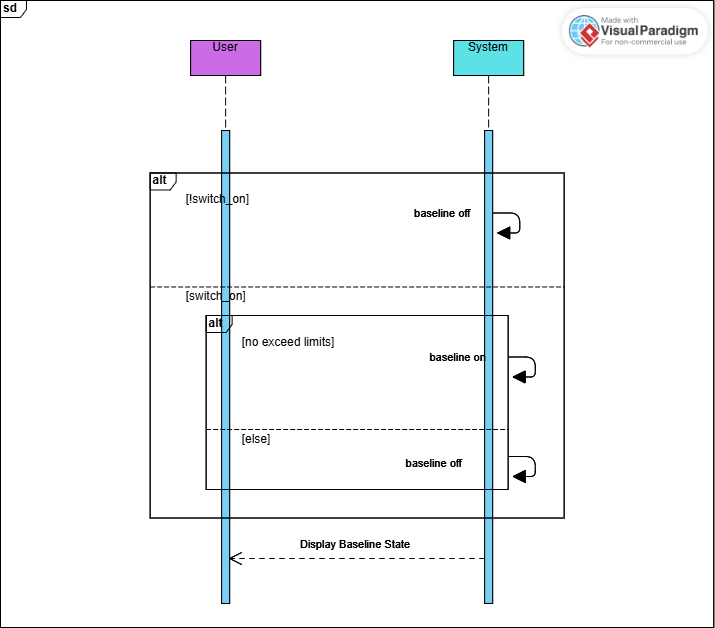
\includegraphics[width=0.8\textwidth]{img/S1_5.png}
  \caption{S1.5}
\end{figure}
Backend: If \lstinline!database.calculate_1h()! plus the next drop amount will exceed 1 or \lstinline!database.calculate_24h()! plus the next drop amount will exceed 3, don't inject. If the switch is off, don't inject. Else inject.

System Response: One line displays the state.
\subsubsection*{S1.6: Reset Injection Records}
Frontend: The user click on the "Reset" button.

Backend: \lstinline!database.baseline_timeline_list! and \lstinline!database.bolus_timeline_list! are set to empty.

System Response: The two progress bars will be empty.
\subsection*{S2: Patient Operations}
\subsubsection*{S2.1: Request Bolus}
\begin{figure}[htbp]
  \centering
  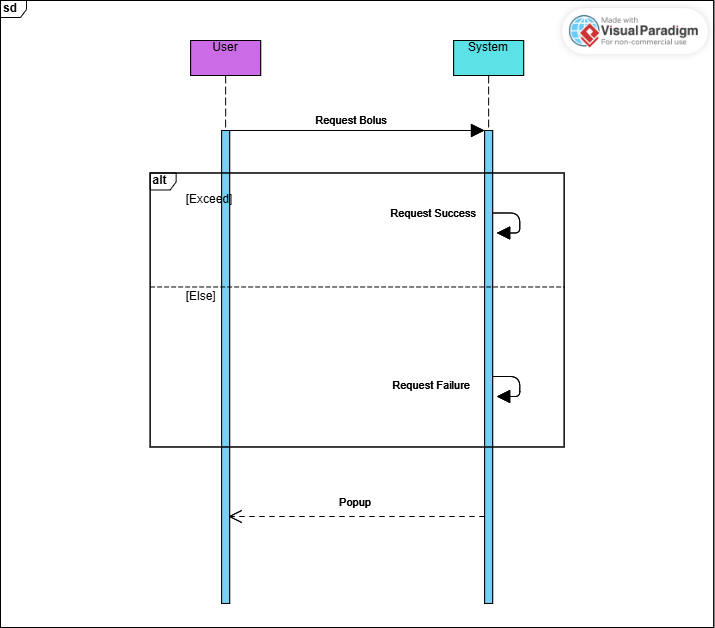
\includegraphics[width=0.8\textwidth]{img/S2_1.png}
  \caption{S2.1}
\end{figure}
Frontend: The user clicks on the "RequestBolus" button.

Backend: If \lstinline!database.calculate_1h()! plus the bolus amount will exceed 1 or \lstinline!database.calculate_24h()! plus the next bolus amount will exceed 3, don't inject. Else inject. A record \lstinline![time,database.bolus_amount]! will be added into \lstinline!database.bolus_timeline_list!.

System Response: Failed or succeeded, a message box will pop up to inform you the detailed information.
\subsection*{S3: Update}
\subsubsection*{S3.1: Update}
Backend: First judge baseline state. If it's being injected, \lstinline!current_injected_amount=database.baseline_amount!, else it's 0.
If \lstinline!database.baseline_timeline_list! is empty, append\lstinline![time,current_injected_amount]!.
Else if append\lstinline![time,current_injected_amount]! is different from the last element in the list, append\lstinline![time,current_injected_amount]!, else pass.

System Response: Update the two progress bars.

\end{document}
